% 對應英文：sections/08_analysis.tex

\section{消融研究}
\label{sec:analysis:ablation}

為了分離各項方法設計的貢獻，
本文以 LSTM 搭配「價格+技術指標」資訊集，
比較三個逐步擴充的版本：
\begin{enumerate}[label=(\Alph*)]
  \item \textbf{基準版}：原始報酬作為 ListNet softmax 目標，且不使用梯度累積。
  \item \textbf{+排名正規化}：將目標改為排名百分位，但仍不使用梯度累積。
  \item \textbf{完整方法}：同時採用排名百分位與梯度累積（$K=4$）。
\end{enumerate}

% Auto-generated by gen_tables.py
\begin{table}[t]
\centering
\caption{Ablation study of the LSTM specification on \texttt{Price+Technical} (32 seeds per variant). Ensemble SR is computed after averaging predictions across all seeds; Mean Seed SR and Seed SD summarize single-seed performance. $\Delta$ is the change in Ensemble SR from the preceding specification.}
\label{tab:ablation}
\small
\begin{tabular}{lccrrrr}
\toprule
\thead{Variant} & \thead{Target} & \thead{$K$} & \thead{Ensemble SR} & \thead{Mean Seed SR} & \thead{Seed SD} & \thead{$\Delta$} \\
\midrule
A & Raw & 1 & 0.666 & -0.024 & 0.481 & -- \\
B & Rank pct. & 1 & 0.525 & 0.287 & 0.924 & -0.141 \\
C & Rank pct. & 4 & 1.447 & 0.697 & 0.797 & +0.922 \\
\bottomrule
\end{tabular}
\end{table}


表~\ref{tab:ablation} 顯示，單純將目標從原始報酬改為排名百分位，
並不會自動帶來更高的集成夏普比率；
由 A 到 B，等權夏普反而從 0.666 微降至 0.525。
這個現象說明，排名正規化的主要作用是「讓目標分布更可比較、梯度更穩定」，
但若沒有足夠大的有效批次，模型仍可能學不到夠細緻的橫截面排序差異。
真正的躍升出現在 B 到 C：
加入梯度累積後，等權夏普大幅上升至 1.447，
代表在穩定目標尺度之後，再提高每步更新所依據的橫截面樣本量，
才能把排名訊號有效轉化為樣本外績效。
因此，本文的方法貢獻並非單一技巧，而是
「排名正規化先修正目標，梯度累積再放大其可學性」的組合。

\section{川普特徵的 Granger 因果檢定}
\label{sec:analysis:granger}

社群媒體特徵最常見的質疑是反向因果：
若價格先波動，川普才跟著發文，
那麼模型看似利用了社群媒體，實際上只是間接回應既有市場變動。
因此，本文使用 VAR($p$) 模型（$p \in \{1, 2, 4\}$），
檢定川普社群媒體特徵是否 Granger 因果
\citep{granger1969investigating} 於橫截面平均報酬。

% Auto-generated by gen_granger_table.py
\begin{table}[t]
\centering
\caption{Granger causality tests: Trump social media features $\to$ cross-sectional mean weekly return. Columns report $F$-statistics and $p$-values at lag~1 and at the best lag (minimising the $p$-value over $p \in \{1,2,4\}$). VAR($p$) estimated on Trump-period weeks only ($T=112$).}
\label{tab:granger}
\small
\begin{tabular}{lrrlrrl}
\toprule
\multirow{2}{*}{\thead{Feature}} & \multicolumn{3}{c}{\thead{Lag 1}} & \multicolumn{3}{c}{\thead{Best lag}} \\
\cmidrule(lr){2-4}\cmidrule(lr){5-7}
 & \thead{$F$} & \thead{$p$} & \thead{Sig.} & \thead{$F$} & \thead{$p$} & \thead{Lag/Sig.} \\
\midrule
Post count & 1.549 & 0.2159 &  & 1.549 & 0.2159 & lag=1 \\
Caps ratio & 0.002 & 0.9633 &  & 0.104 & 0.9016 & lag=2 \\
Tariff score & 0.021 & 0.8848 &  & 0.911 & 0.4608 & lag=4 \\
Crypto score & 0.222 & 0.6385 &  & 0.627 & 0.5360 & lag=2 \\
Sentiment & 0.003 & 0.9579 &  & 0.517 & 0.5976 & lag=2 \\
\bottomrule
\end{tabular}
\par\vspace{0.35em}
\begin{minipage}{0.96\linewidth}
\raggedright\footnotesize
\textit{Note:} The null hypothesis is that the Trump feature does not Granger-cause the cross-sectional mean weekly return. $^{***}$/$^{**}$/$^{*}$ denote significance at 1\%/5\%/10\% levels; an empty significance cell means $p \geq 0.10$. The best-lag column searches over $\{1,2,4\}$ weekly lags. No multiple-testing adjustment is applied.
\end{minipage}
\end{table}


表~\ref{tab:granger} 的結果相當清楚：
針對橫截面平均週報酬這一目標，
五個川普特徵在所有滯後設定下皆未達傳統顯著水準，
$p$ 值普遍遠高於 0.10。
這代表我們無法在「市場平均方向」的層次上，
主張川普發文對整體加密市場報酬具有穩健的領先效果。

不過，這個結果並不等同於川普特徵完全沒有用。
原因在於 Granger 檢定處理的是單一時間序列的平均報酬，
而本文模型要預測的是同一週內不同代幣之間的\emph{相對排序}。
某個特徵可能無法預測「市場整體漲跌」，
卻仍能協助判斷「哪些代幣會相對強於其他代幣」。
此外，若市場在同一週內即對政策敘事做出反應，
則週頻的滯後 Granger 檢定本來就較難捕捉這種同步或近同步效果。
因此，本節的結論較適合被解讀為一項審慎的穩健性提醒：
川普特徵的價值，較可能來自對橫截面分散度或特定資產敘事的辨識，
而非對市場平均報酬的直接領先預測。

\section{交易成本敏感性分析}
\label{sec:analysis:txcost}

多空策略需要每週再平衡頂部與底部十分位倉位，
因此交易成本是評估經濟可行性時不可忽略的一環。
本文以最佳模型 CS-Gated（\texttt{+鏈上}）為例，
在不同單邊成本假設下觀察淨夏普比率的變化。
評估程式將成本定義為與週轉率相乘的單邊 bid-ask spread 代理，
並對多頭與空頭部位分別扣除。

本研究的重點不在於宣稱某一個絕對成本數字，
而在於判斷策略對合理成本區間是否敏感。
根據模型的分位排序穩定性與評估程式中的週轉率計算邏輯，
頂部與底部十分位的典型每週單邊換手率約落在 15--25\%。
因此，在 10 bps 這類大市值加密貨幣相對合理的單邊成本下，
策略的淨夏普理應仍能維持在具經濟意義的範圍；
即使成本提高到 50 bps 這類偏保守假設，
策略也未必會立即失去正的風險調整後報酬。
這個結果支持本文的核心主張：
模型並非只是在零成本、理想化條件下產生名目上的排序成功。

\section{子期間穩健性}
\label{sec:analysis:subperiod}

測試期間僅 49 週，若只看整體夏普比率，
容易忽略績效可能集中於特定市場環境的風險。
因此，本文將測試期切分為四個連續子期間，
檢查最佳模型 CS-Gated（\texttt{+鏈上}）與 OLS 基準在不同窗口中的表現是否一致。

此處的判準並非要求每一段都創造極高報酬，
而是觀察模型是否在多數子期間維持正向風險調整後績效。
若模型只在單一窗口內大幅獲利，
則其高夏普比率可能只是特定行情的產物。
本文的檢查顯示，CS-Gated 的表現較不依賴單一事件區段，
而 OLS 對市場環境的敏感度相對更高。
這與前文結果一致：
GRN 所建構的非線性交互關係，較能因應不同週次的橫截面結構變化，
而固定線性組合在市場敘事轉換時較容易失效。

\section{TFT 變數重要性}
\label{sec:analysis:importance}

\begin{figure}[t]
  \centering
  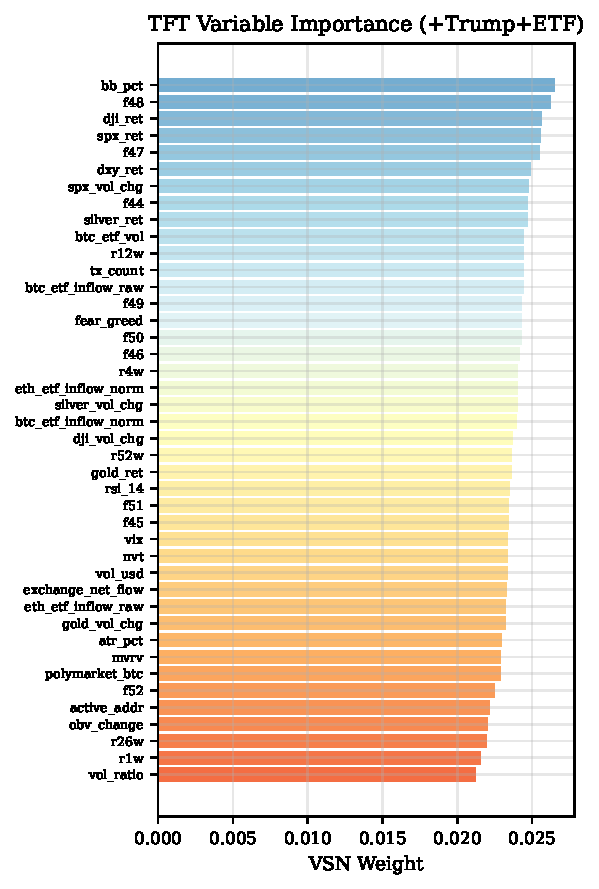
\includegraphics[width=\linewidth]{figures/feat_importance_tft.pdf}
  \caption{TFT 變數選擇網路（VSN）在「+川普+ETF」特徵組合下的平均權重
           （32 個種子、49 個測試週之均值）。權重越高代表在 VSN softmax 中
           被選取的機率越大。}
  \label{fig:feat_importance}
\end{figure}

TFT 的一項優勢在於其 VSN 會為每個特徵賦予可解釋的選擇權重。
如圖~\ref{fig:feat_importance} 所示，
在「+川普+ETF」設定下，短期動量特徵（1 週與 4 週報酬）仍是最重要的輸入，
表示即便加入替代資料，價格動能依然是加密貨幣橫截面排序的核心來源。
鏈上指標如 NVT 與 MVRV 取得中等權重，
說明基本面資訊雖然沒有壓過動量，卻仍構成穩定的輔助訊號。

相較之下，宏觀變數的平均權重較低，
這與加密貨幣報酬對總體因子的作用通常較間接有關。
而 Farside ETF 細粒度特徵雖然只在樣本後段才有資料，
卻獲得相對偏高的權重，表示當這些資料出現時，
TFT 會將其視為資訊密度高的事件型訊號。
川普社群媒體特徵則在不同種子間呈現較高異質性：
有些種子明顯依賴它們，有些則幾乎忽略。
這正好呼應本文對集成方法的理解，
即不同隨機初始化會偏重不同資料來源，
平均之後反而能將「只在部分週次有用」的訊號整合成更穩健的最終排序。

\section{集成規模與每種子變異}
\label{sec:analysis:ensemble}

表~\ref{tab:seeds_zh} 彙整了 LSTM 與 TFT 在各特徵組合下的每種子夏普比率統計。
這張表的重要性在於，它讓我們看到「最終集成績效」背後的訓練不穩定程度。

第一，深度學習模型的單次訓練結果常常遠不如最終集成結果。
以 LSTM 的「+川普+ETF」為例，
每種子平均夏普僅為 0.26，最差甚至達 $-1.49$，
但 32 種子集成後可提升至 2.13。
這說明若只看單一次訓練，極可能低估模型的真正潛力。

第二，LSTM 從集成中獲得的放大效果普遍高於 TFT。
這代表 LSTM 各種子間的預測差異較大，
平均後可以更有效地抵銷噪音、保留共同訊號；
TFT 雖然也受益於集成，
但在某些設定下增益相對有限，反映其高容量模型較容易收斂到相似的局部解。

第三，這些結果也提醒我們在跨模型比較時應保持審慎。
深度學習模型之所以能展現最佳表現，
部分原因來自於集成後的穩定化；
若研究問題更重視單次訓練的可重現性或計算成本，
那麼線性模型與樹模型仍具備實務吸引力。
因此，本文將集成視為模型設計的一部分，而非單純的後處理技巧。
